\section{Parsing Vue.js}

\subsection{Assumptions}
It is assumed that the Vue.js code, for which interaction diagrams are going to be generated, compiles and does not contain syntactical errors. No checks are performed in order to verify that. Naturally, logical errors are not an issue.
\subsection{Limitations}
\label{concept:parsing_limits}

In order to be able to generate interaction diagrams, which capture every aspect of Vue.js, the generation must be directly based on an \gls{ast}, which covers every possible syntax, such as \cite{eslint_vue_parser}. 

The approach proposed here only includes the following features of Vue.js:
\begin{itemize}
    \item Event handlers (including anonymous method syntax and method reference syntax)
    \item Any one or two-way binding expressions (\code{v-model}, \code{v-bind}, "moustache", \code{v-if}) excluding \code{v-else}
    \item \code{v-for} statements for lists, excluding iterating through properties of an object or iteration with index (property zipped with index)
    \item distinguishing between properties and computed properties
    \item complex object and lists (non-nested) models 
    \item methods, including the resolution of arguments, they have been called with (excluding methods called with other methods as arguments)
\end{itemize}

\subsection{AST}

\begin{lstlisting}[language=antrl]
grammar vue_simple;

program: bindings methodDefinitions createdMethod topLevelProperties computedProperties;

topLevelProperties: thisIdentifier*;
methodDefinitions: methodDefinition*; 
createdMethod: methodDefinition;
computedProperties: (methodDefinitionIdentifier reads writes calls)*;

methodDefinition: methodDefinitionIdentifier methodArgs reads writes calls;

methodArgs: NAME_IDENTIFIER*;
reads: accessedVariable*;
writes: accessedVariable*;
calls: calledMethod*;

calledMethod: calledMethodIdentifier '(' calledArgs ')';
accessedVariable: identifier;
calledArgs: (calledMethod | accessedVariable)*;

bindings: binding*;
binding: tag bindingSource+;
bindingSource: (accessedVariable | calledMethod) (EVENT_BINDING | ONE_WAY_BINDING)
                | accessedVariable TWO_WAY_BINDING;

tag: name tagId loc;
tagId: LINE '_' COLUMN '_' LINE '_' COLUMN;
name: UNICODE | identifier;
loc: start end;
start: LINE COLUMN;
end: LINE COLUMN;

calledMethodIdentifier: methodDefinitionIdentifier | id* NAME_IDENTIFIER;

methodDefinitionIdentifier: THIS NAME_IDENTIFIER;
thisIdentifier: THIS identifier;
identifier: NAME_IDENTIFIER id*;


id: NUMERIC_INDEX | GENERIC_INDEX | NAME_IDENTIFIER;

//terminals, tokens
LINE: [0-9]+;
COLUMN: [0-9]+;

EVENT_BINDING: 'event';
TWO_WAY_BINDING: 'two-way';
ONE_WAY_BINDING: 'one-way';

GENERIC_INDEX: 'i' | 'j' | 'k' | 'l' | 'm' | 'n';
THIS: 'this';

NUMERIC_INDEX: [0-9]+;
NAME_IDENTIFIER:  JS_IDENTIFIER;
JS_IDENTIFIER:  (UNICODE | '$' | '_') (UNICODE | '$' | '_' | [0-9])*;
UNICODE: [\u0000-\uFFFF];
\end{lstlisting}
\label{ast}

A Vue.js \gls{spa}, including all the necessary information for \ref{concept:parsing_limits}, can be defined using the above grammar. 

The application consists of \code{bindings} \code{methodDefinitions} a \code{createdMethod}, \code{topLevelProperties} and \code{computedProperties}. 

The \code{topLevelProperties} represent the \code{data} object of the Vue.js \code{script} tag. Each property will be represented flattened, as a list of identifiers and prefixed with \code{this},in order to indicate it belongs to the top level data object. For example \code{problem:\{a:0, b:0\}} will be represented as follows:

\begin{figure}[H]
    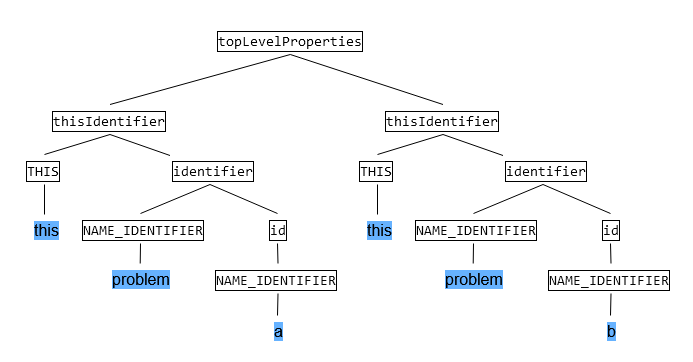
\includegraphics[width=0.8\textwidth]{images/ast_top_level.png}
     \caption{\gls{ast} for top-level example }
     \label{fig:ast_top_level}
\end{figure}

Bindings can be obtained from the Vue.js \code{template}.

Each binding consists of an HTML tag, an a list of binding sources for that tag - pairs of variable or method call and a binding type. The binding type represents the type of the binding - either event, one-way or two-way. Two-way bindings are only valid with properties, whereas for events and one-way bindings, both method calls and properties are possible, since in Vue.js a binding source could be an expressions defined as an inline anonymous functions (
    \code{<div v-if=\"value === true\"/>}
). The binding sources are a list, since a tag could have multiple different bound properties, or a bound expression. The information about how exactly the properties are bound, if it is the same type of binding, is discarded.

Method calls include the parameters they have been called with - other methods or just variables. It is also possible to call methods with binary expressions - those are represented as a special method, which takes 2 parameters - the left and right side operators of the binary expression. Expressions with multiple terms can be represented as multiple binary expressions. This representation loses information such as the order of operations, but since we are only interested in which properties are being accessed, this loss does not pose an issue.

A special case is accessing lists. For example \code{<div v-bind="problems[0].a"/>} would result in the following:

\begin{figure}[H]
    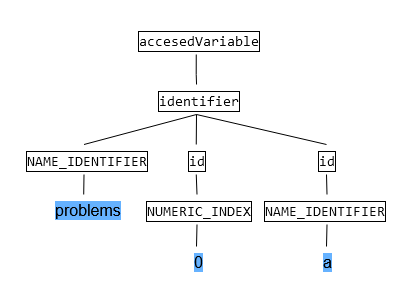
\includegraphics[width=0.8\textwidth]{images/ast_problems_0_a.png}
     \caption{\gls{ast} for example }
     \label{fig:ast_list_simple}
\end{figure}


\code{v-for} statements, are substituted:
\begin{lstlisting}[style=html]
<ul>
  <li v-for="subject in subjects" :key="subject.id">
    {{ subject.problems[0] }}
  </li>
</ul>
\end{lstlisting}
results in
\begin{lstlisting}[style=html]
subjects[i].problems[0]
\end{lstlisting}
which in term produces the following AST:

\begin{figure}[H]
    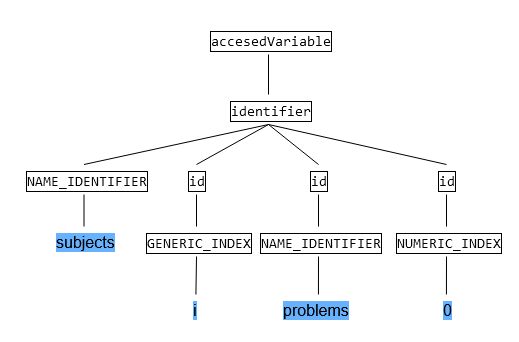
\includegraphics[width=0.8\textwidth]{images/ast_numeric_generic.png}
     \caption{\gls{ast} for example }
     \label{fig:ast_list_complex}
\end{figure}

Nested lists are also possible and would result in multiple generic indices being added.

Each tag includes its location in the source code (starting and ending line and column), which can also be used as an identifier. Tags also have humanly readable names, which are either equal to the the text of the tag, if it exists, or to the identifier of the first binding. 

\code{methodDefinitions} include all methods definitions from the \code{method} object of the \code{view-model}. Each method definition consists of the following
\begin{itemize}
    \item identifier - an identifier, equal to \code{this} followed by the name of the method
    \item arguments - names of arguments, each of which is a simple name identifiers
    \item reads - variable it reads from
    \item writes - variables it writes to
    \item calls - method calls, including arguments, same as for bindings 
\end{itemize}

\code{computedProperties} are similar to \code{methodDefinitions} with the exception that they do not have arguments. Albeit bad practice, it is still possible for computed properties to have side effects and therefore they were modelled as methods.

%%%%%%%%%%%%%%%%%%%%%%%%%%%%%%%%%%%%%
%                                   %
%   Interaction Diagram Generation  %
%                                   %
%%%%%%%%%%%%%%%%%%%%%%%%%%%%%%%%%%%%%
\section{Interaction Diagram Generation}

The simplified Vue.js \gls{ast} can be used to create a directed graph, which will represent the interaction diagrams. It is hard to directly generate this graph, therefore the capabilities of a directed, \gls{compound_graph} graph will be leveraged and later on converted to a directed graph. 

Vertices in this graph have the following properties
\label{concept:interaction_diagram_structure}
\begin{enumerate}
    \item \gls{guid} - used to reference and globally identify the vertex 
    \item \code{label} - the name of the vertex, which is going to be displayed
    \item \code{type} - the type of the vertex (data, tag or method). Additionally for data vertices: numeric, generic or undefined (representing simple data vertices)
    \item \code{loc} - defined only on tag vertices. Their location in the source code
    \item \code{parent} - defined only on vertices of type 'data'. A \gls{guid} of another vertex, used for a child/parent relationship (compound graph).
\end{enumerate}

Edges in the graph are directed and each have a label property, which is one of 'event', 'calls' or 'simple'. 

The core idea of the algorithm is to generate vertices only for nodes which are being accessed instead of the whole application. A second pass of the data is also needed to add additional edges for lists. 

\subsection{Variable Identifiers}
\label{concept:variable_identifiers}
Variable identifiers are represented by \astnode{identifier} and \astnode{thisIdentifier} in the \gls{ast} \ref{ast}. For the \astnode{this} and for each \astnode{id} node in the \astnode{identifier} or \astnode{thisIdentifier} a vertex is created in order. 
Those vertices are connected using unidirectional edges, labeled with 'data' and also each vertex (excluding the first one) has its parent set to the previous. There is one exception to this process - When accessed from \astnode{write} of a \code{method}, nodes of type \astnode{GENERIC_INDEX} are omitted. The reason behind this will be explained in this section \ref{concept:why_create_list};


Each vertex has a \gls{guid} equal to the value of its terminal symbol (\astnode{NUMERIC_INDEX}, \astnode{GENERIC_INDEX} or \astnode{NAME_IDENTIFIER}), concatenated with the value of the previous vertex.
The \code{label} of those vertices are equal to the terminal symbol in case of \astnode{NAME_IDENTIFIER} and in case of \astnode{GENERIC_INDEX} and \astnode{NUMERIC_INDEX}, combined with the \code{label} of the previous vertex using square braces. Set the type of each vertex to 'data'. Add the type 'numeric' to vertices created from \astnode{NUMERIC_INDEX} nodes and 'generic' to vertices created from \astnode{GENERIC_INDEX} nodes. 

\begin{figure}[H]
    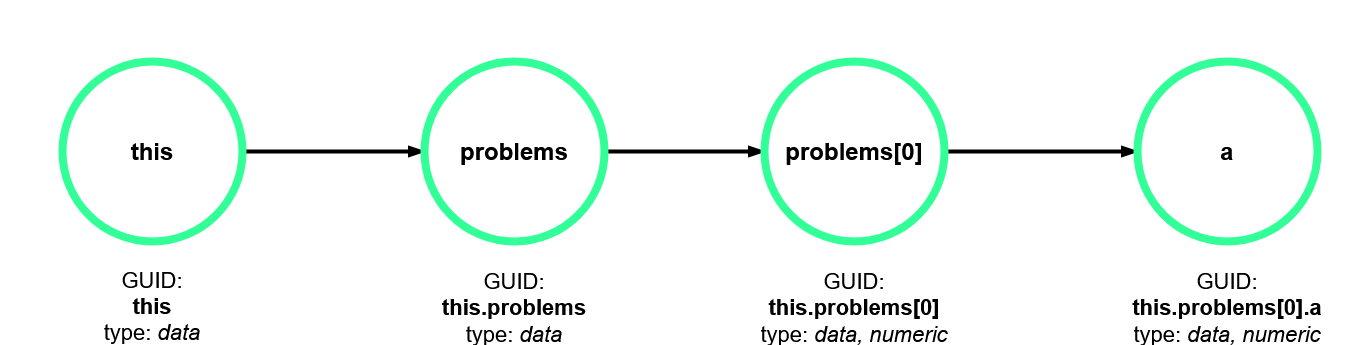
\includegraphics[width=0.8\textwidth]{images/graph_simple.png}
     \caption{Example Graph obtained for the identifier \code{this.problems[0].a} }
     \label{fig:graph_simple}
\end{figure}

\subsection{Object representation}

Using the representation for identifiers in the previous section, objects will result in being displayed dynamically, based on which properties are accessed. Nodes and edges are created on a 'create if non-existent' basis. In the example below, if \code{this.problem.b} is accessed after \code{this.problem.a} it will only result in the creation of the node \code{a} and edge \code{this.problem} -> \code{this.problem.b}.

\begin{figure}[H]
    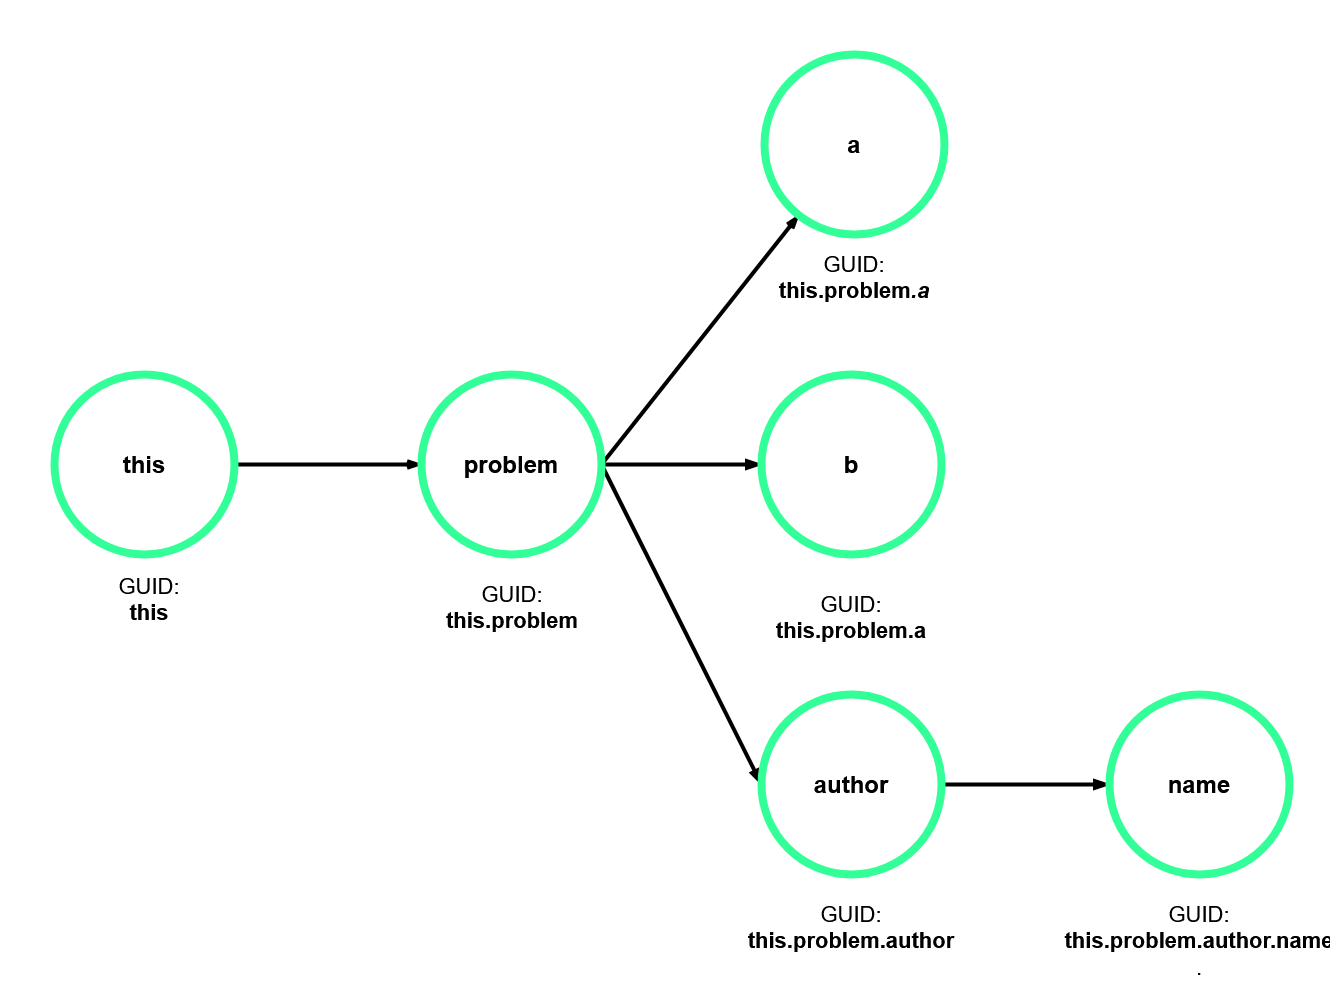
\includegraphics[width=0.8\textwidth]{images/graph_object.png}
     \caption{Example Graph for the following object accesses - \code{this.problem.a}, \code{this.problem.b},  \code{this.problem.author.name} }
     \label{fig:graph_object}
\end{figure}

Furthermore, updates can be formulated nicely with the above representation. If \code{problem} were to be changed, it would result in a cascade update of all properties. If \code{author} would be change, it would only result in a cascading change in \code{name}. 

\subsection{List representation}
\label{concept:list_creation}

Lists will be represented based on the template in \ref{fig:graph_list_generic} for a list named $P$.  %TODO for a list named $P$ don\tlike this
\begin{figure}[H]
    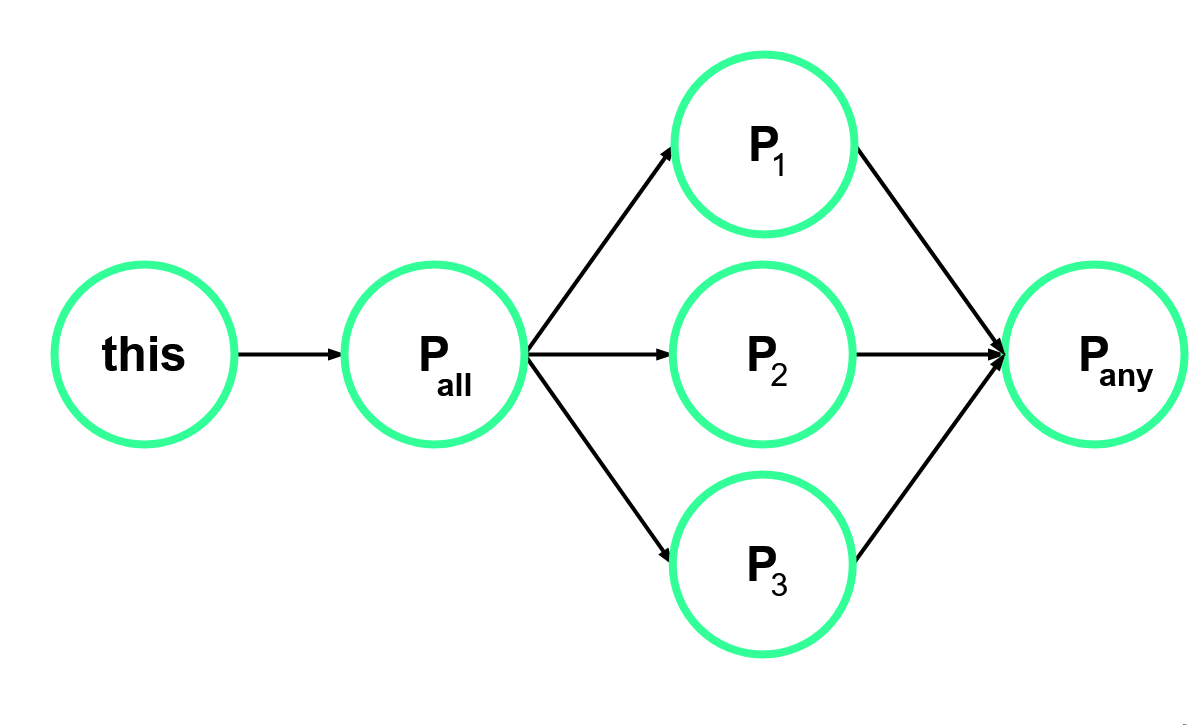
\includegraphics[width=0.8\textwidth]{images/graph_list_generic.png}
     \caption{Generic List representation}
     \label{fig:graph_list_generic}
\end{figure}

Concrete elements, which are accessed, are denoted as $P_{<index>}$ and additionally a vertex $P_{all}$, which can be used to update all elements of a list\label{concept:why_create_list} and their properties, is created. Another vertex $P_{any}$ is also created, which can be used to observe once any vertex of $P_1$, $P_2$, $P_3$, \dots $P_n$ changes. If $P_1$ were to be updated by any method, it would not result in updates to any of $P_2$, $P_3$, \dots $P_n$

The same construct can also be leveraged when it comes to properties of list elements. Each top level property of that element will have an $all$ vertex, connected to the $P_{all}$ node of the list.  

\begin{figure}[H]
    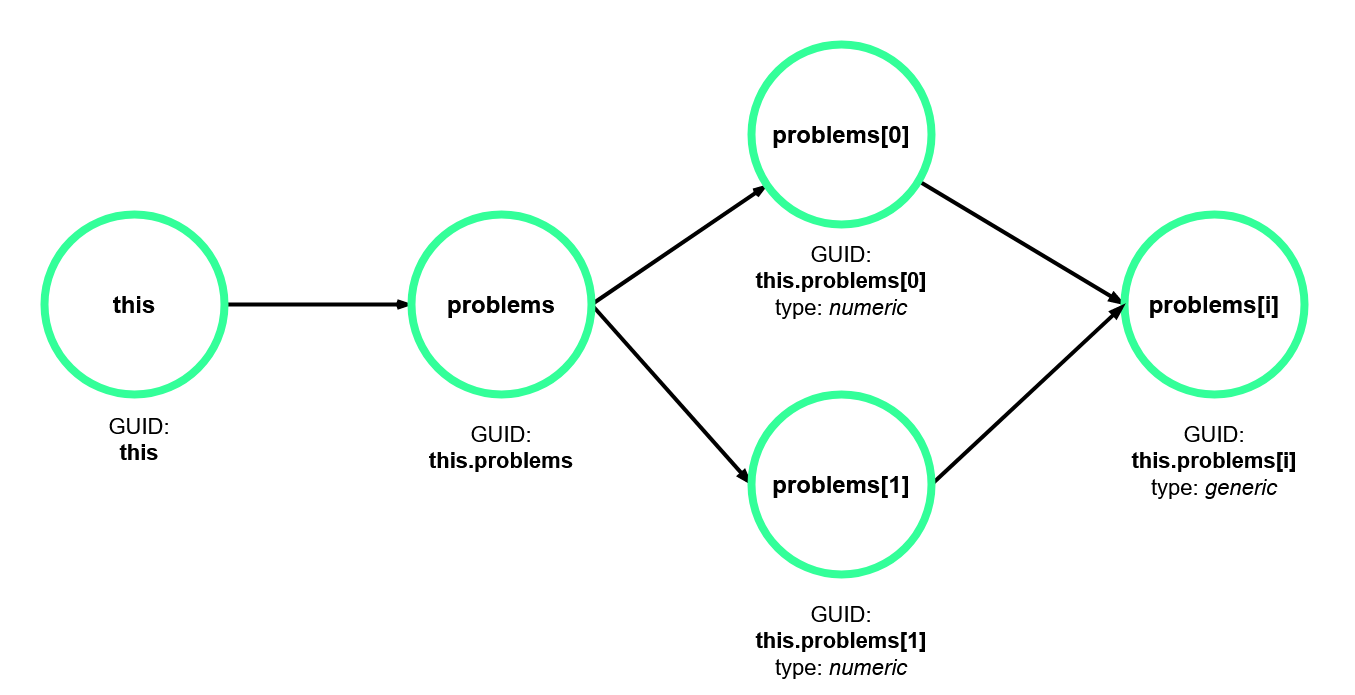
\includegraphics[width=0.8\textwidth]{images/graph_list.png}
     \caption{Concrete example of a list representation}
     \label{fig:graph_list}
\end{figure}

\subsection{Method representation}
\label{concept:methods}
Methods have two related \gls{ast} nodes - \astnode{methodDefinition}, representing the definition of a method and \astnode{calledMethod} representing a call of a method. 

First it should be determined if a vertex needs to be created for an \astnode{calledMethod} node. This is done by looking up based on the name of the \astnode{calledMethod} in \astnode{methodDefinition}, ignoring \astnode{THIS}. If the lookup is successful a vertex should be created as described below. If not, it should be checked if the method is a method call on a top level property instance. This can be done by comparing if it starts in the same way as one of \code{topLevelProperties}. %TODO that's not so clear an a bit slapped here. check tomorrow
If that's the case, it is assumed, that it mutates whole property and the method should instead be treated as a write operation.
If both of the above fail, the called method does not belong to context and is of no interest.

The next step is to resolve the names of the arguments it has been called with \astnode{calledArgs}. Every argument, that can neither be found in \astnode{computedProperties} nor \astnode{topLevelProperties} is replace by a fixed word such as $OTHER$ or $*$. In order to obtain the \gls{guid} of the vertex, the name of the \astnode{methodDefinitionIdentifier} is taken, \astnode{THIS} is excluded, and concatenated with the the resolved arguments, which are joined with $,$ and surrounded with brackets. The \code{label} of this node is equal to its name, excluding \astnode{THIS} from arguments. 

The vertex for the method call is now completed. Multiple calls of this method with the same arguments will all result in the same vertex.

Now vertices for nodes the method interacts with, based on its \astnode{methodDefinition}, have to be created. Those include the variables it reads - \astnode{reads}, and writes - \astnode{writes} and methods it calls - \astnode{calls}. 

Firstly, the arguments from the \astnode{methodDefinition} need to be substituted with the resolved arguments the method was actually called with and update all \astnode{reads}, \astnode{writes}  \astnode{calls} referencing them. All of them, which do not start with \astnode{THIS} can be discarded, since they do not belong to the context. Once filtered out, create a list of vertices for each variable in \astnode{reads} and \astnode{writes} as described in \ref{concept:variable_identifiers} and connect the most precise of those (the last of each list) to the method vertex. For the vertices resulting from \astnode{writes}, this edge has a label of 'writes' and the property vertex as the source and method vertex as the sink. For the vertices resulting from \astnode{reads}, this edge has the method vertex as the source and property vertex as the sink. 
Finally the process described in this section is repeated recursively for each \astnode{calledMethod} node in \astnode{calls} and an edge labeled 'calls' is added from the current method vertex to the resulting ones. 

\subsubsection{Computed property representation}
\label{concept:computed_property}

Computed properties are represented similarly to methods, except they cannot have arguments, so no substitution of arguments is required. When defining their \code{label} and \gls{guid} both are equal to the \astnode{methodDefinitionIdentifier}. \astnode{reads}, \astnode{writes} and \astnode{calls} are computed in the same manner as methods. 

\subsubsection{Combining it all together}
\label{concept:algorithm_create_diagrams}

Interaction diagrams can be generated from the simplified Vue.js \gls{ast} in the following way:

%TODO how to indent
For each \astnode{binding} in \astnode{bindings}:
- for each \astnode{tag}, \astnode{bindingSource}  in \astnode{binding}:

Create a vertex for \astnode{tag}, with a \gls{guid} \astnode{tagId} and label \astnode{name} and type 'tag'.

if the \astnode{binding} is an \astnode{accessedVariable}, determine if it is a computed property by looking it up in \astnode{computedProperties} and if so, treat it as a computed property, and create vertices as described in \ref{concept:computed_property}. Otherwise determine if it as top level property, by doing a lookup on \astnode{topLevelProperties}, treat it as a property and create vertices for it as described in \ref{concept:variable_identifiers}. In either cases, connect it to the \astnode{tag} vertex, based on the binding type. If the \astnode{accessedVariable} is neither, it does not belong to context and can be discarded. %TODO YADA YADA, ignore this prefix when checking

if the \astnode{binding} is an \astnode{calledMethod} create a vertices for it as described in \ref{concept:methods}. Connect it to the \astnode{tag} vertex, based on the binding type.

Based on binding type, the following edges are created:
A) If the binding type is an event binding, create an 
edge with the tag vertex as a source and the binding vertex as sink and label it 'event'. 
B) If the binding type is one-way, create an edge with the binding vertex as source and the tag vertex as sink.
C) If the binding type is two-way, create both edges - A) and B).

For the initial method - \astnode{createdMethod}, create a vertex with \gls{guid} and name equal to \textit{created} and create vertices for its \astnode{reads}, \astnode{writes} and \astnode{calls} analogous to methods as described in \ref{concept:methods}. 


Once all of the above is done, additional edges will need to be added for the \textit{all} vertices of properties of elements inside lists \ref{concept:list_creation}. Also the edges to the \textit{any} vertex will be missing. 

'numeric' vertices to the 'generic' one. 

This is achievable by first finding all vertices of type 'generic' or 'numeric' and obtaining the parent of each of them. Those parents form a subset of all vertices, that have have 'generic' or 'numeric' vertices as children and additionally other properties (properties on list elements, with $type(v) \neq generic, type(v) \neq numeric$). 
For each of those parent vertices $p$:
Firstly, connect each 'numeric' vertex to the 'generic' one. Recursively connect each child in the tree of the 'numeric' vertex to the child of the tree of the 'generic' vertex with the same name. If either does not exist, no edge is created. Do the same for $p$ and all 'numeric' vertices and the 'generic' vertex.

\begin{figure}[H]
    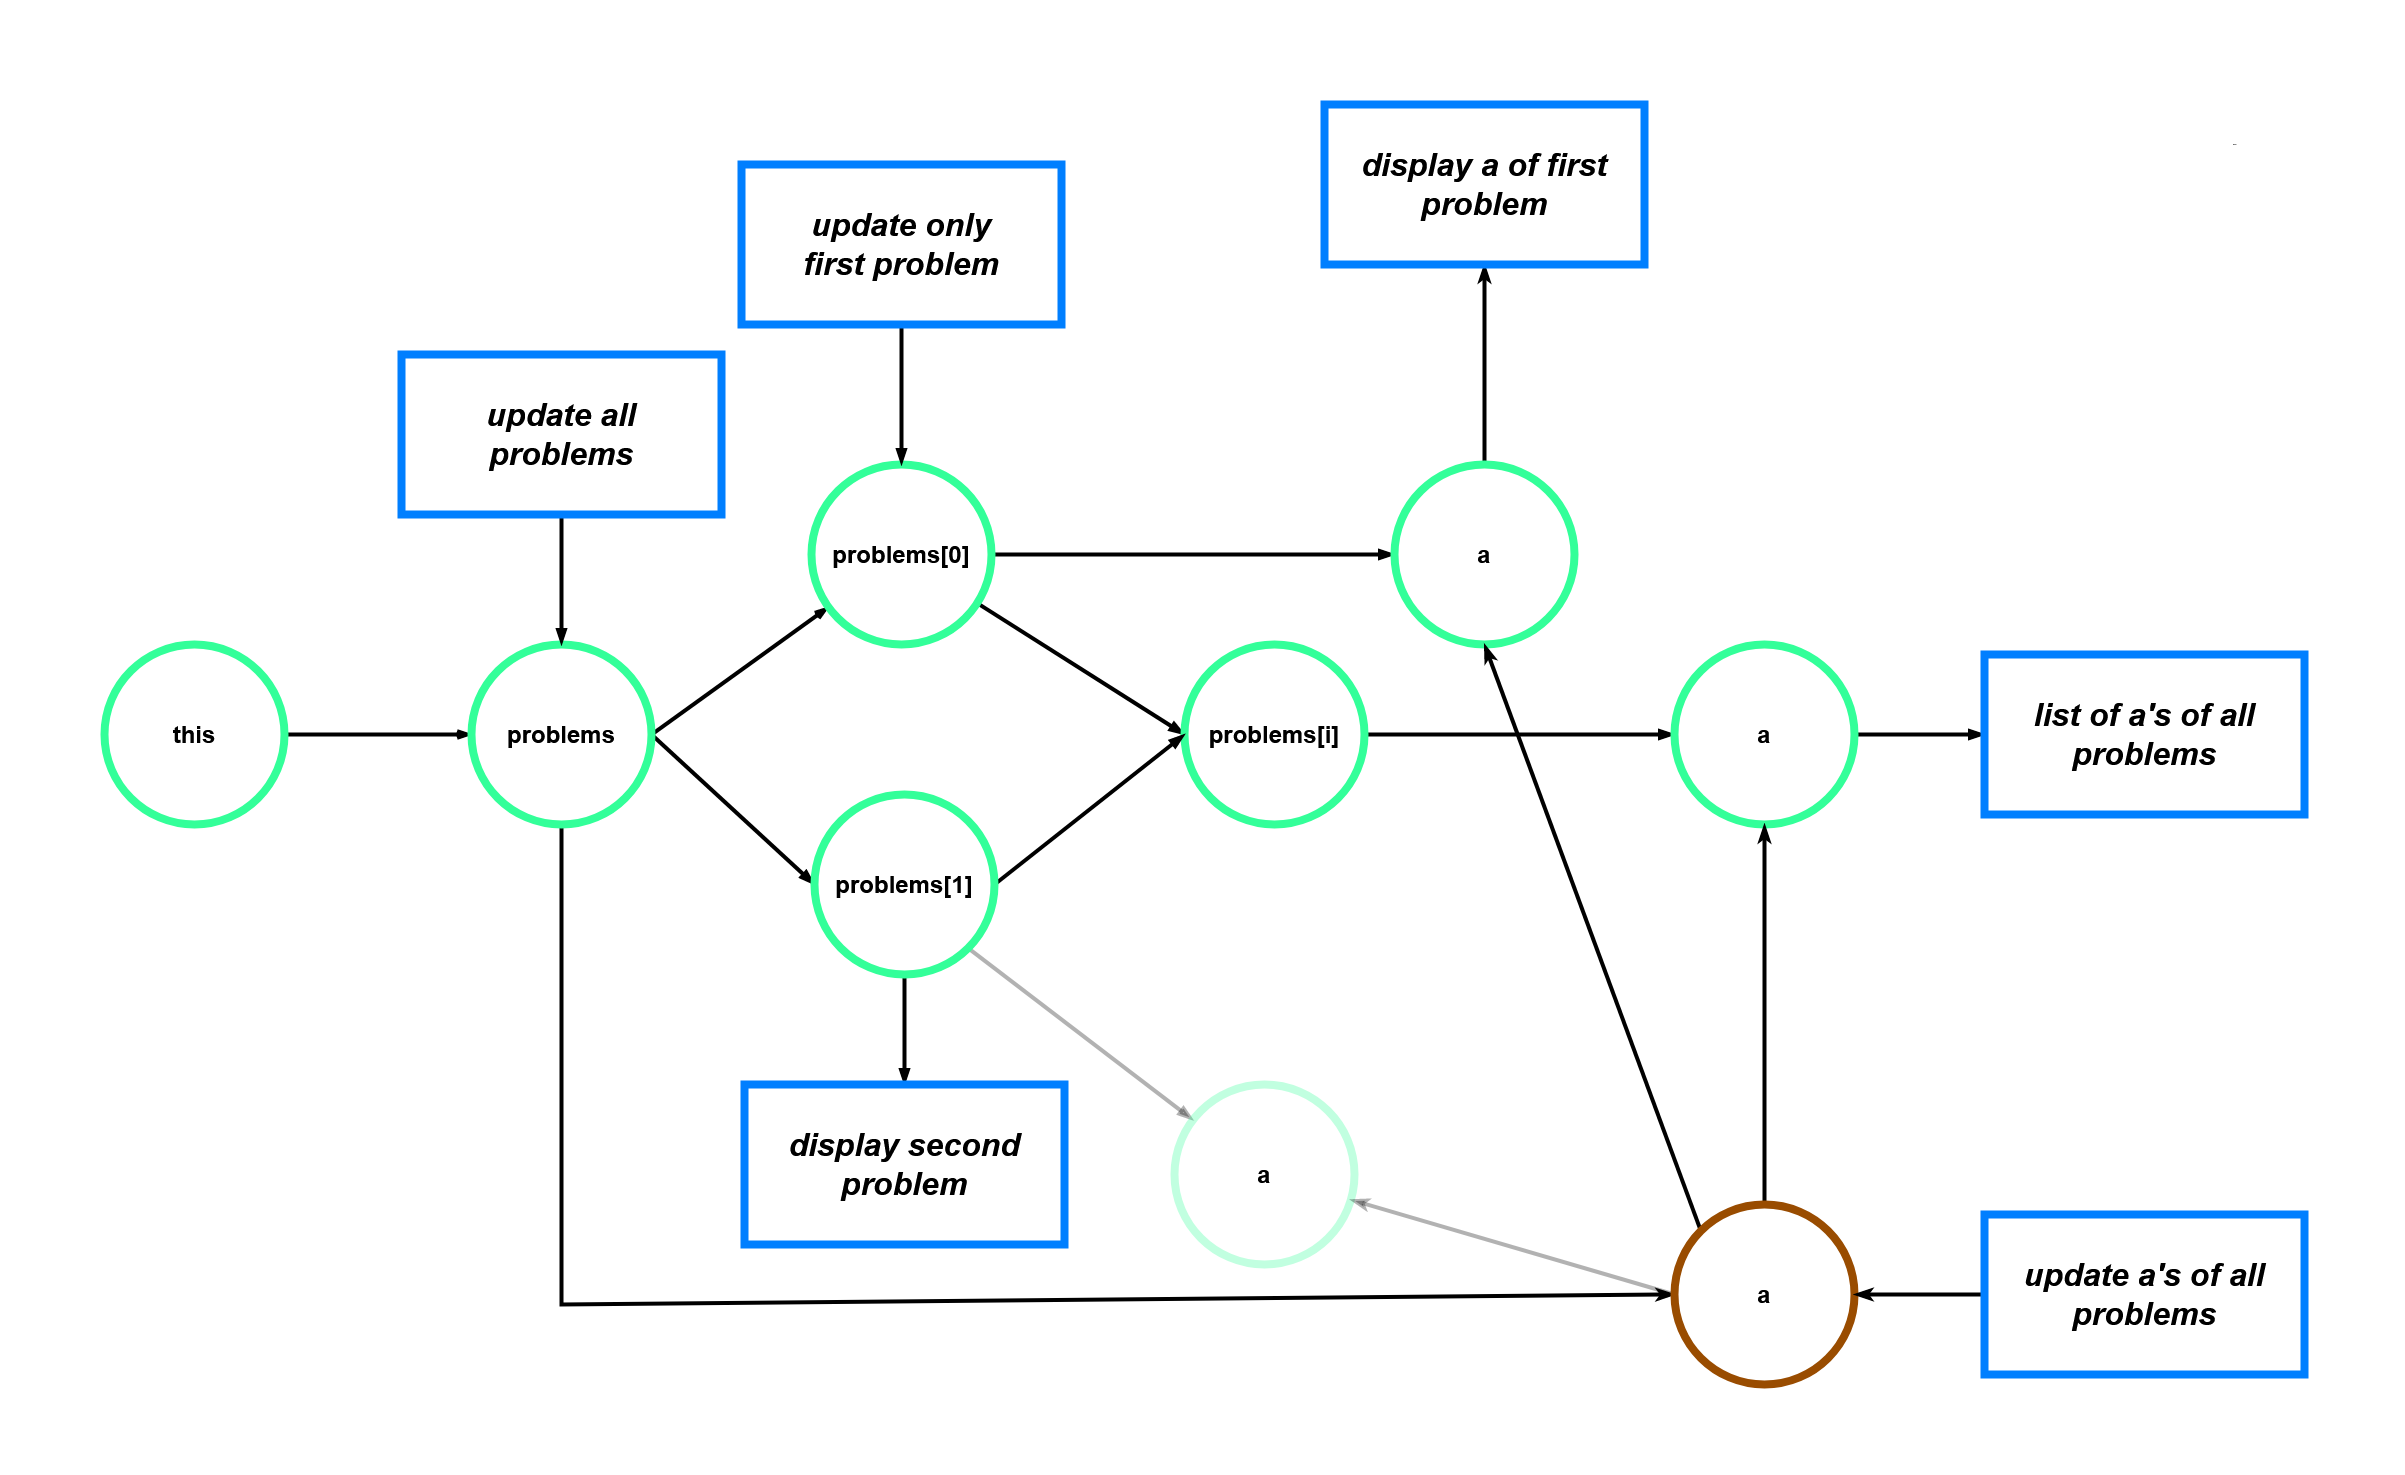
\includegraphics[width=0.8\textwidth]{images/graph_complete_example.png}
     \caption{Example Graph including list elements with properties}
     \label{fig:graph_complete_example}
\end{figure}

%TODO describe this and also verify above
\section{Scenario Generation}
\label{concept:scenario_generation}
In order to generate scenarios in Gherkin, interactions can be sliced in a similar manner as described by \textcite{zhang2019scenario} and summarized in \ref{intro:zhang_interaction_diagrams}.

Let $N$ denote the set of all nodes in the graph and $E$ denote all edges in the graph. Let $n \in N$, $m \in N$ be any two nodes in the graph and $(n, m) \in E $ represent an edge from $n$ to $m$. Let $type(n)$ be a function, that returns the type of a node and $label(n, m)$ be a function that returns the label of the edge from $n$ to $m$. Let $E_{out}(n)$ be a function, which returns all outgoing edges of $n$.
Let $E_{in}(n)$ be a function, which returns all incoming edges to $n$.

Let $N_I$ denote all nodes, that the user can interact with. A node $n \in N$ is also in $N_I$ if $\exists e \in E_{out}(n)$ where $label(e) = event$. Let $N_H$ denote all html tag nodes. A node $n \in N$ is also in $N_H$ if $type(n) = tag$. 
Given a node $n_H \in N_H \cup {created}$, a node $m_H \in N_H$ reacts to $n_H$ iff
\begin{enumerate}
    \item $\exists n_0,n_1,n_2, \ldots,n_k \in N, n_0=n_H,n_k=m_H$ such that for each $0 \leq i < k  $ $(n_i,n_{i+1}) \in E$, and $label(n_i,n_{i+1})\neq event$ and if $label(n_i,n_{i+1}) \neq calls$ $\forall n_{i+1_{in}} E_{in}(n_{i+1})$ $label(n_{i+1_{in}}) \neq event$ 
\end{enumerate}

Analogous to \cite{zhang2019scenario} let $l(n)$ denotes all nodes, that react to $n$. A sequence of user interactions, starting with the initial function is referred to as a \textit{scenario} $A=(a_0,a_1,\ldots, a_n)$ where $a_0=created$ and $\forall0 < k \leq n, a_k \in N_I$. 
Define the HTML tags, to which a scenario reacts, to be equal to the tags to which the last tag in the scenario reacts $l(A)=l(a_n)$. Define a function that returns the last element in a scenario - $last(A) = a_n$

The set of scenarios is generated by starting with the initial scenario, containing only the initial function $S_0 = \{(created)\}$. It is then prolonged by all tags $n \in N_I$, representing that the user can click anywhere. For further steps, only tags, that can be updated are included, so additionally $n \in l(A)$ must hold. The newly included tag should also not be the same as the last element of the scenario, which means that also $n \neq last(A)$ must hold.
Formally:
Define $A \oplus x = a_0,a_1,\ldots,a_n,x$. Then
\begin{align}
    S_n = \begin{cases} 
        \{(created)\} &\mbox{if } n = 0 \\
        \{ p \oplus x |p \in S_{n-1}, x \in \mathcal{I}\} &\mbox{if } n = 1 \\
        \{ p \oplus x |p \in S_{n-1}, x \in l(p) \cap \mathcal{I}, x \neq last(p) \} 
    \end{cases}
\end{align}
This is repeated up to $k$ times, where $k$ is a constant set by the user. 

A Gherkin scenarios templated can then be obtained by the following template:

Scenario - $n_0,n_1 \ldots n_k$

Given - $n_0, n_1 \ldots n_{k-1}$

When - $n_k$

Then - $l(n_k)$


%TODO dynamically and then connect idea

%lists better explain, generic acts as the any, etc.